\documentclass[12pt]{article}

%packages go here!
\usepackage{anyfontsize}
\usepackage{tikz} %For drawing the cover page's background
\usepackage{graphicx}
\usepackage{titlesec}
\usepackage[a4paper, 
	right=2cm,
	left=4.3cm,
	top=2.25cm, bottom=1.25cm]{geometry}
\usepackage[document]{ragged2e} %Left alignment
\usepackage{parskip} %Add an additional line after paragraphs
\usepackage{fancyhdr} %Put numbering on top
\usepackage{enumitem} %List handling
\usepackage{caption} %Caption handling
\usepackage{layout} %Printing out the layout for debugging

%Setting the font
\renewcommand{\rmdefault}{phv} % Arial
\renewcommand{\sfdefault}{phv} % Arial

%Enter parameters here
\newcommand\myauthor{Vo Dang Khoa(T5616SN)}
\newcommand\mytitle{An Arbitrary tilte goes here!}
\newcommand{\subtitle}{Some subtitle goes here!}
\newcommand{\rpas}{Report or Assignment}
\newcommand{\course}{Course name}

\linespread{1.5}

%Redefining maketitle
\renewcommand{\maketitle}{
\thispagestyle{empty}

\begin{center}

\fontsize{16}{19} \selectfont \myauthor

\vspace{20pt}

\MakeUppercase{\fontsize{24}{30} \selectfont \mytitle}

\vspace{5pt}

\fontsize{20}{25} \selectfont \subtitle

\vspace{20pt}

\fontsize{16}{19} \selectfont {\rpas \\ \course}

\vspace{20pt}

\the\year

%Adding the logo
\vspace{100pt}

\includegraphics{logo.jpg}

\end{center}

%Making the cover background
\tikz[remember picture,overlay] \node[inner sep=0pt] at (current page.center){

\includegraphics[width=\paperwidth,height=\paperheight]{coverbg.png}};
\clearpage
}

%Formatting The sections:
\titleformat{\section}
{\bfseries}
{\thesection}
{.17in}
{\MakeUppercase}

%The subsection:
\titleformat{\subsection}
{\bfseries}
{\thesubsection}
{.17in}
{}

%Formatting the paragraphs
%Put new line between paragraphs
\setlength{\parskip}{\baselineskip}
%No indentation
\setlength{\parindent}{0pt}

%Content of the document
\begin{document}
%The cover page
%First we must clear up the margin
\newgeometry{
	right=2cm,
	left=2cm,
	top=4cm,
	bottom=2cm,
	}
{\maketitle}

%Table of content:
\thispagestyle{empty}
{\tableofcontents}

{\clearpage} %% old habits die hard ;-)

%Formatting the margin for the rest of the document
%(If 'restoregeometry' doesn't work then I have no other options":
\newgeometry{
	right=2cm,
	left=4.3cm,
	top=2.25cm,
	bottom=2.5cm,
	}

%Put numbering on top (i.e. the header)
\pagestyle{fancy}
\fancyhf{}
\chead{\thepage}
\renewcommand{\headrulewidth}{0pt} %No line please!
%Format the footer also while we're at it:
\renewcommand{\hoffset}{2in}

%Formatting lists:
\setlist[itemize]{leftmargin=.6in, nosep} %Vertical spacing of list paragraphs is none

%Caption handling:
\captionsetup[figure]{font=small, position=below}
\captionsetup[table] {font=small, positiona=above}
%The below line was marked with "b"
%===========================================================================================================
%CONTENT GOES HERE!
\section{Introduction}
This template for writing reports or assignments at Xamk was last updated on 16 August 2017. The template has been optimised for full, downloadable version of Microsoft Word – not for wordprocessing applications such as Office 365 operating in the cloud.

\section{Layout of reports of assignments}
This chapter introduces the layout of text produced with the template. Appendix 1 
provides more information on the technical details of this template.

\subsection{Title page, table of contents, margins, indentation, fonts, font sizes 
and page numbers}

The layout of the title page, table of contents and list of references do not require students’ own work. The example information of the template can simply be replaced by the details of each report or assignment. Automatic hyphenation can be disabled in the title of the title page.

The title page follows the layout of the title page in this document. The title page includes the student’s own name, the title of the report or assignment, the type of the document − for example practical training report or learning diary − and the date of the report or assignment. There is no page number on the title page, and reports or assignments 
do not include abstracts and forewords or prefaces. 

The heading of the table of contents is CONTENTS, and page 2 of this document shows an example. If the report of assignment does not include numbered headings, the table of contents is not needed. Its purpose is to introduce the overall outline of the document and make it easier to read. Therefore, the table of contents has different heading levels to indicate heading hierarchy. It shows the heading words together with the number of the page where the text under each heading starts. The numbering and headings in the table of contents are identical to the ones used in the main body of the text. If the table of contents is generated with the wordprocessor’s function, this tool automatically updates the changes made in the text into the table of contents. Appendix 1 provides instructions for using these update functions. The table of contents also includes the heading REFERENCES, and the headings LIST OF FIGURES or LIST OF TABLES and APPENDICES, if necessary, but they are not numbered as chapters. In addition, the page number for the table of contents is not displayed on the page.

Uncommon characters and symbols, terms, self-made symbols and abbreviations can be listed separately. This list of definitions is placed after the table of contents and before the introduction without a page number. Its heading does not have a number, but it is listed in the table of contents. Standard symbols and abbreviations and common scientific terminology do not require definitions. Characters, terms, symbols and abbreviations can also be explained in the text. In this case, no separate list of definitions is necessary.


\textbf{Font and font sizes:}

\begin{itemize}
	\item{headings and body text with Arial, font size 12}
	\item{captions for figures and tables with Arial, font size 10}
\end{itemize}

\textbf{Margins}

\begin{itemize}
	\item{right margin 2 cm}
	\item{left margin 4.3 cm}
	\item{top margin 2.25 cm}
	\item{bottom margin 1.25 cm}
	\item{body text with line spacing 1.5}
	\item{captions for figures/tables and appendices with line spacing 1}
\end{itemize}

Both headings and text lines start at the left margin without indentation. The style selected for writing body text is Normal. This ensures that the text is automatically indented correctly and that line spacing remains at 1.5. There should be an empty line before each paragraph. The key used for starting a new paragraph is Enter, and this key is not used for line breaks. If a manual line break is necessary, it is done with the key combination Shift+Enter.

The text is written with automatic hyphenation and aligned left. There is no need for alignment on the right. The text should not have incomplete pages between chapters, but proceeds in an uninterrupted flow of chapters and sections. However, an isolated heading at the end of a page should be moved on to the following page.

The automatic numbering function is used for page numbers. They are placed at the top centre approximately 1 cm from the top of the paper. The page number count begins from the title page, but page numbers are only displayed from the introduction chapter onwards.

Appendices do not necessarily have a running page number. Instead, they are numbered by adding the word Appendix, together with the relevant ordinal number, in the right top corner of the page, as shown in Appendix 1, for example. There is no full stop after the ordinal number. Appendices with multiple pages are introduced for instance with Appendix 1/2, where the first number indicates the number of the appendix and the second the page number. In other words, Appendix 1/2 refers to the second page of the first appendix. (See Appendices 1/1 and 1/2.)

\subsection{Headings and the table of contents}
It is recommended to update the headings and table of contents of this template by using the update functions of Word. Appendix 1 provides instructions for updating the table of contents and for creating new headings.

There is an empty line before and after all headings and they have numbers as well. These same numbers also automatically appear in the table of contents when using the Styles tool of Word. The type of heading determines which heading style of Word to select: Heading 1 is used for main headings and Heading 2 for subheadings. Heading 3 is used for further subheadings, if necessary. This three-step heading hierarchy is usually sufficient. Too detailed hierarchy could result in too short and list-like passages of text. In addition, isolated, numbered subheadings should be avoided: If the text has subheading 7.2.1, there should also be 7.2.2.

\subsection{Figures and tables}
Figures and tables can be used to illustrate some of the data introduced in the text. The words used in referring to these are \textbf{Figure} and \textbf{Table}. Other possible words, such as graph, chart or illustration should not be used. Figures and tables should include explanations for all the symbols used in them.

The term Figure refers to graphs, charts, photographs, drawings, screen shots and graphical presentations. All figures and tables must be informative and technically accurate. They are incorporated in the body text, if they essentially relate to the text and are not very large in size or number. Large figures or tables and series of figures or tables with many items are placed in the appendices. Tables provide exact illustration, while figures are more expressive. Drawings should be produced by following the field-specific instructions and standards. In case of large volume of figures or tables, it is typical to introduce them in separate lists of figures or tables placed between the list of references and appendices. Appendix 3 provides instructions for drawing up a list of figures or tables. To ensure that the size of the report or assignment files remains reasonable, figures should be compressed. Information on compression is available in Appendix 1. 

Tables are used to present series of numbers and large quantities on data. Their columns have headings and sufficient commentary to make the tables understandable independent of the text. Readers should be able to interpret the tables reading only the row and column texts, together with the captions.

There are separate numbers for tables and figures (Table 1, Table 2, Figure 1, Figure 2 etc.) running throughout the text. A caption is added for each of them, and this also applies to formulas, as shown in Appendix 2. Captions can be like headings or consist of one or more sentences. The figure caption is placed below the figure, whereas a table caption is placed above the table. The first word in the caption is written with a capital initial. After that lower-case letters are used, unless grammatical reasons require capital initials, as with proper nouns and adjectives referring to nationalities and languages, for example. Captions are written with Arial and font size 10, and the line spacing for captions with multiple lines is 1. Word functions should be used for inserting the numbers and figure and table captions, and there are instructions for this in Appendix 1.

The text should include references to all tables and figures with their appropriate numbers. Other types of references, such as the following figure, on the previous page, should be avoided. Figure 1 below shows two possible techniques for referring to figures and tables.

\textbf{Reference can be incorporated in the sentence structure:}

\textit{”Figure \ref{bacpic} illustrates the thesis process from idea to publication. The process has been divided into phases of 5 ECTS credits and it is supported by reporting and feedback.”}

\textbf{Reference can be introduced in brackets:}

\textit{”The thesis process can be divided into five phases, including idea, planning, implementation, assessment and publication (Figure \ref{bacpic}).”}

\begin{figure}
	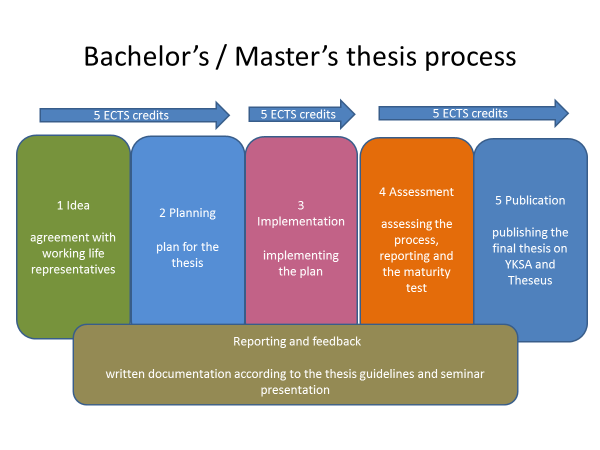
\includegraphics{Figure1.png}
	\caption{Figure 1. Bachelor’s / Master’s thesis process (Heikkinen et al. 2013)\label{bacpic}}
\end{figure}

Reference alone is not enough, but the body text should also explain the figures and tables, so that readers can understand their main message based on the text. The symbols used must follow the standards and be consistent with the ones used in the text. If the date presented in a figure or table has been taken from another source, the caption must mention that source according to Xamk’s Referencing guidelines available at the Student intranet. Figure 1 above includes this kind of reference.

As already mentioned, figures and tables must always be discussed in the body text. They can never start a chapter, but should always be preceded by an introduction in the text. For example, a figure is preceded by an explanation and followed by an interpretation. If the same figure is mentioned later in the text, the reference can include the page number for the figure as follows (Figure \ref{bacpic}, page \pageref{bacpic}). No figure or table can form a chapter, nor end it.




















\end{document}
